\documentclass[report,paper=b5,fontsize=13Q]{jlreq}

\usepackage{luatexja-otf}
\usepackage[sourcehan-jp,no-math,match,deluxe,jfm_yoko=jlreq]{luatexja-preset}

\usepackage{graphicx}
\usepackage[svgnames]{xcolor}
\usepackage{float}
\usepackage{mathtools,amssymb,amsthm}
\usepackage[unicode,hidelinks,pdfusetitle]{hyperref}
\usepackage{cleveref}
\usepackage{makeidx}
\usepackage{subfiles}

\usepackage{geometry}
\usepackage{tocloft}
\usepackage{floatflt}
\usepackage{subcaption}
\usepackage{enumitem}
\usepackage{pdfpages}

\usepackage{listings}
\usepackage{pgfplots}
\usepackage{tcolorbox}
\usepackage{xparse}
\usepackage{bxghost}
\usepackage{mathpunctspace}
\usepackage{bxtexlogo}
\usepackage{lipsum}
\usepackage[ISO]{diffcoeff}
\usepackage{comment}

% パッケージの初期設定
\usetikzlibrary{graphs,cd,datavisualization.formats.functions}
\tcbuselibrary{xparse,listings,breakable,skins,theorems}
\pgfplotsset{width=7cm,compat=1.18}
\bxtexlogoimport{*,SATySFi}
\makeindex

% メタデータ
\title{\TeX/\LaTeX ことはじめ}
\author{cuttlefish\_math}
\date{\today}

% レイアウト操作
\geometry{b5paper,hmargin=15mm,vmargin=20mm}
\setsansjfont{Source Han Sans JP Regular}[YokoFeatures={JFM=jlreq},BoldFont={Source Han Sans JP Medium}]
\setmonofont{HackGen Regular}[BoldFont={HackGen Bold}]
\renewcommand{\cfttoctitlefont}{\sffamily\Huge\bfseries}
\renewcommand{\cftchapfont}{\sffamily\bfseries}
\renewcommand{\cftchappagefont}{\sffamily\bfseries}
\setlength{\cftchapnumwidth}{4\zw}
\newcommand{\idxdelim}{\hfill}
\newcommand{\makeidxhead}[1]{{\vbox{\hbox to \linewidth{\sffamily\bfseries #1\hfill}}}\nopagebreak}

% 参照
\crefname{theorem}{定理}{定理}
\crefname{definition}{定義}{定義}
\crefname{example}{例}{例}
\crefname{lemma}{補題}{補題}
\crefname{section}{節}{節}
\crefname{subsection}{小節}{小節}
\crefname{table}{表}{表}
\crefname{figure}{図}{図}

% ソースコード
\definecolor{codeback}{HTML}{EEEEEE}

\lstdefinestyle{codeblock}{%
  aboveskip=0pt,
  belowskip=0pt,
  breaklines=true,
  breakindent=10pt,
  basicstyle=\ttfamily\small}

\newtcblisting{codeblock}{%
  listing only,
  listing options={style=codeblock},
  enhanced,
  breakable,
  colback=codeback,
  arc=0mm,
  boxrule=0mm,
  top=2mm,
  bottom=2mm,
  left=2mm,
  right=2mm,
  frame hidden}

\NewDocumentCommand{\inlinecode}{O{!} v}{\eghostguarded{}\lstinline[breaklines=true,basicstyle=\ttfamily]#1#2#1\eghostguarded{}}

% 定理環境
\theoremstyle{definition}

\tcbset{%
  myframe/.style={%
    colframe=gray,
    boxrule=0.2mm,
    arc=0mm,
    boxsep=0mm,
    left=0mm,
    right=0mm,
    top=0mm,
    bottom=0mm},
  mystyle/.style={%
    enhanced,
    label type={#1},
    theorem style=plain,
    fonttitle=\bfseries,
    colframe=black,
    colback=white,
    colbacktitle=white,
    coltitle=black,
    enlarge top by=0.6\zh,
    arc=0mm,
    boxrule=0.2mm}}

\newtcbtheorem[number within=section]{theorem}{定理}{mystyle={theorem}}{theorem}
\newtcbtheorem[number within=section]{definition}{定義}{mystyle={definition}}{definition}
\newtcbtheorem[number within=section]{lemma}{補題}{mystyle={lemma}}{lemma}
\newtheorem{example}{例}[section]

% グラフ
\tikzset{%
  hv path/.style={to path={-| (\tikztotarget)}},
  vh path/.style={to path={|- (\tikztotarget)}},
  terminal/.style={%
    rectangle,
    minimum size=6mm,
    draw=black!50},
  mapping/.style={%
    rectangle,
    minimum size=6mm}}

% マクロ(文書構造)
\newcommand{\smallfiguresize}{5cm}
\newcommand{\figuresize}{7cm}
\newcommand{\termdef}[1]{{\sffamily\bfseries #1}}

% マクロ(数式)
\providecommand\given{}
\DeclarePairedDelimiterX{\Set}[1]{\lbrace}{\rbrace}{\renewcommand\given{\nonscript\:\delimsize\vert\allowbreak\nonscript\:\mathopen{}}#1}
\newcommand{\literal}[1]{\mathrm{#1}}

\begin{document}
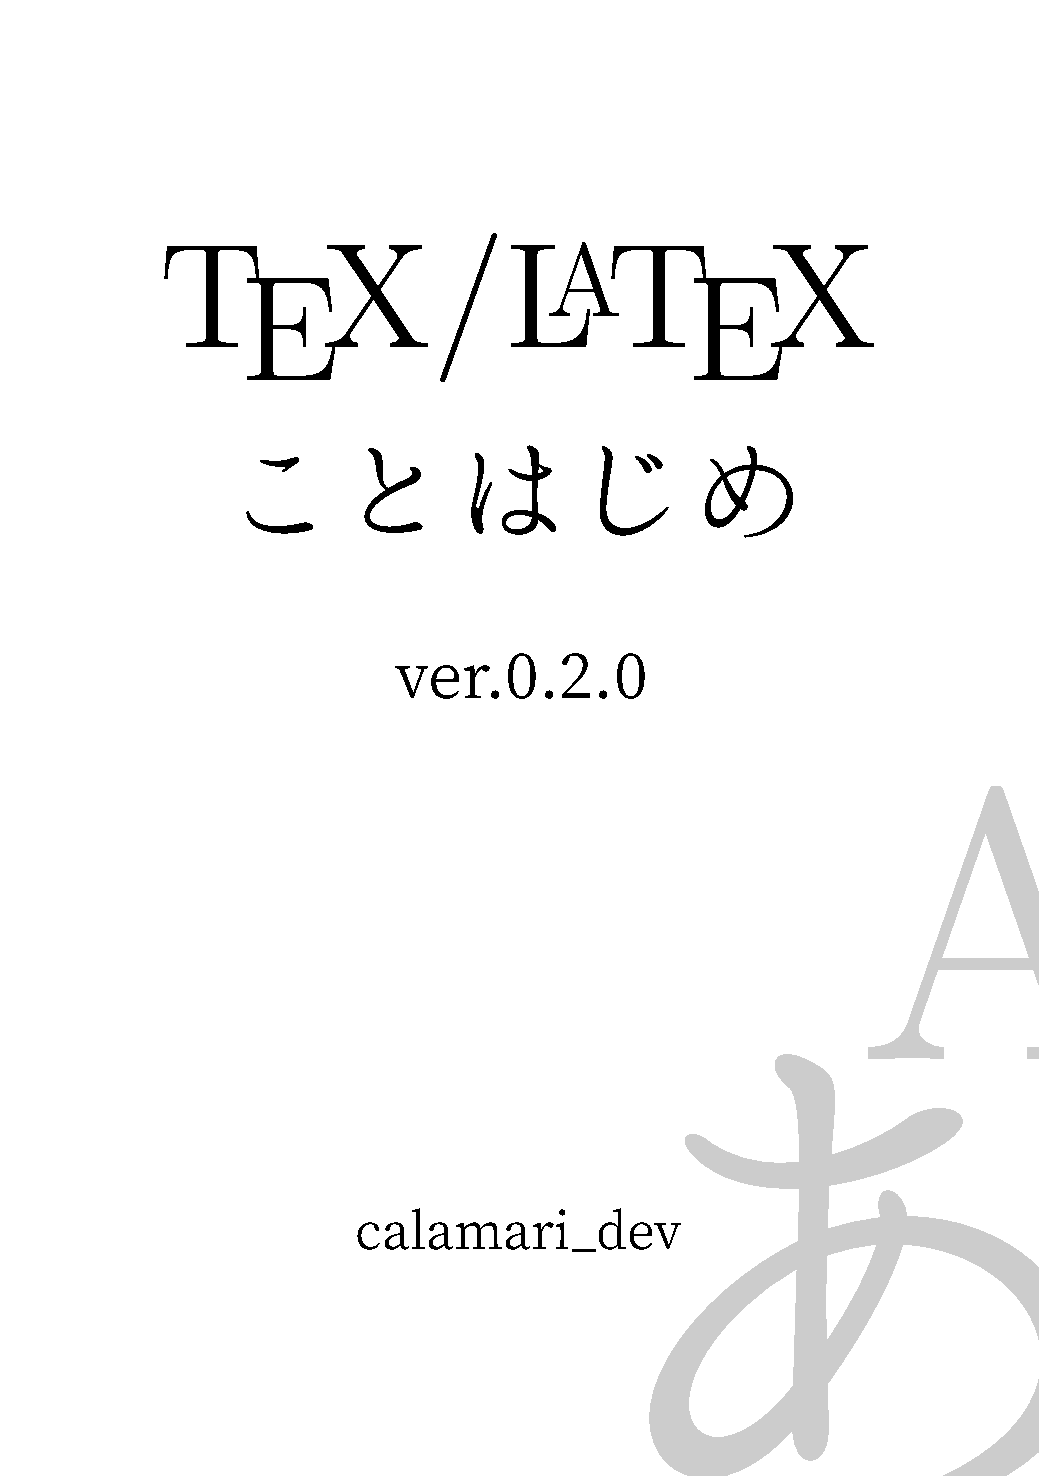
\includepdf{titlepage.pdf}
\tableofcontents

\subfile{chapter/in_the_beginning}

\subfile{chapter/computer_and_multimedia/index}

\subfile{chapter/what_is_texlatex/index}

\subfile{chapter/graph/index}

\chapter{フォント}
この節では処理系を\LuaTeX に限定する.これは,\LuaTeX が日本語組版に対応しており,
かつフォントを簡単に変えられる処理系だからである.

\LuaTeX において,和文フォントの変更は\inlinecode{luatexja-fontspec}\index{luatexja-fontspec@luatexja-fontspec}パッケージにより行う.
たとえば,この文書ではプリアンブルに次のように書くことで,ソースコードのフォントを白源\footnote{\url{https://github.com/yuru7/HackGen}}に変更している.
\begin{codeblock}
\setmonofont{HackGen Regular}[BoldFont={HackGen Bold}]
\end{codeblock}

\chapter{補遺}
\section{パッケージの相性問題}
\begin{enumerate}
  \item cleverefはamsmathの後に読み込まれなければならない
  \item hyperrefはxcolorの後に読み込まれるとxcolorの色指定を利用できる
  \item geometryはhyperrefの後に読み込まれなければならない(あるいはgeometryにhyperrefオプションを渡す)  
  \item hyperrefを読み込んだ場合,namerefは\inlinecode{\begin{document}}の直前に読み込まれる
\end{enumerate}

これを見ると分かるが,特にhyperrefに関するものが多い.

hyperref
\begin{quotation}
The environments equation and eqnarray are not supported too well. For example, there might
be spacing problems (eqnarray isn't recommended anyway, see CTAN:info/l2tabu/, the situation
for equation is unclear, because nobody is interested in investigating). Consider using the environments that package amsmath provide, e.g. gather for equation. The environment equation can
even redefined to use gather:
\begin{codeblock}
\usepackage{amsmath}
\let\equation\gather
\let\endequation\endgather    
\end{codeblock}
\end{quotation}

\clearpage
\bibliography{index}
\bibliographystyle{jplain}

\printindex

\end{document}
